% Alloy section, to be included in RASD.tex

\section{Formal Analysis Using Alloy}
\label{sect:alloy}
This section describes the model defined through the Alloy language\textsuperscript{\cite{alloy}}. It is used to define the subset of the domain used to handle tickets, that represents the most critical portion of the system. 

As it can be noted in Section \ref{sect:run}, the chosen bitwidth is 7, thus allowing the generation of integers between $-64$ and $+63$ to meet all constraints.

% FIle to host alloy signatures, to be included in alloy.tex

\subsection{Signatures}
\begin{lstlisting}[language=alloy]
	// Ticket states
	enum State {
		ENQUEUED, 
		CANENTER, 
		DEQUEUED, 
		INSIDE, 
		COMPLETED, 
		WRONG
	}
	
	// All clients of stores
	sig Customer {
		tickets: set Ticket,
		visits: set Visit,
		insideStore: lone Store
	}
	
	// Store signature
	sig Store {
		capacity: one Int,
		delayWindow: one Int,
		queue: one Queue,
		inside: set Customer,
		hours: set OpeningHours
	} {
		capacity > 0
		delayWindow > 0
		#inside =< capacity 
	}
	
	// Signature containing sequences of tickets
	sig Queue {
		store: one Store,
		tickets: seq Ticket
	}
	
	// Ticket signature
	sig Ticket {
		nOrder: one Int,
		customer: one Customer,
		queue: one Queue,
		state: one State
	} {
		nOrder >= 0
	}
	
	// Signature representing a visit that occurred
	sig Visit {
		customer: one Customer,
		accessreq: one Ticket,
		store: one Store,
		weekday: one Int,
		datetimeIN: one DateTime,
		datetimeOUT: one DateTime
	} {
		weekday >= 1 and weekday =< 7
		accessreq.queue.store = store
		accessreq.customer = customer
		isBefore[datetimeIN.time, datetimeOUT.time]
		datetimeIN.time != datetimeOUT.time
	}
	
	// Stores' opening hours
	// In order to simplify the model, 
	// no store is open during day changes
	sig OpeningHours {
		weekday: one Int,
		openingTime: one Time,
		closingTime: one Time
	} {
		weekday > 0 and weekday =< 7
		isBefore[openingTime, closingTime]
		and (openingTime.hours != closingTime.hours 
			or openingTime.minutes != closingTime.minutes)
	}
	
	// Signature used to model time
	sig Time {
		hours: one Int,
		minutes: one Int
	} {
		hours >= 0 
		hours < 24 
		minutes >= 0 
		minutes < 60
	}
	
	// Signature to model a date 
	// (to simplify the year is assumed as 2020)
	sig Date {
		month: one Int,
		day: one Int
	} { 
		month >= 1 and month =< 12
		day >= 1
		(month = 4 or month = 6 or month = 9 or month = 11) 
			implies day =< 30
		else (month = 2) 
			implies day <= 29
		else day =< 31
	}
	
	// Union of date and time
	sig DateTime {
		date: one Date,
		time: one Time
	}
\end{lstlisting}
% Alloy facts, to be included in alloy.tex

\subsection{Facts}

\begin{lstlisting}[language=alloy]
	// Fact to define ticket unicity in queues
	fact uniqueTicketInQueue {
		// No different tickets having the same number
		no disj t, t': Ticket | all q: Queue |
			t in q.tickets.elems 
			and t' in q.tickets.elems
			and t.nOrder = t'.nOrder
		
		// No ticket is in a queue more than once
		all q: Queue | !q.tickets.hasDups
	}
	
	// Facts modeling necessary relations between signatures
	fact implications {
		// Customer <=> Ticket
		all c: Customer | all t: Ticket | 
			t in c.tickets iff t.customer = c
		
		// Customer <=> store
		all c: Customer | all s: Store | 
			s = c.insideStore iff c in s.inside
		
		// Queue <=> Store
		all q: Queue | all s: Store | 
			q.store = s iff s.queue = q
		
		// Queue => Ticket
		all t: Ticket | all q: Queue | 
			t in q.tickets.elems implies t.queue = q
		
		// Visit <=> Customer
		all v: Visit | all c: Customer |
			v.customer = c iff v in c.visits
	}

	// A ticket can correspond to at most one visit
	fact oneTicketPerVisit {
		no disj v,v': Visit | 
			v.accessreq = v'.accessreq
	}
	
	// A customer cannot request a ticket for a store 
	// they are already enqueued for
	fact noSameCustomerInQueue {
		all q: Queue | no disj t, t': Ticket |  
			t in q.tickets.elems 
			and t' in q.tickets.elems 
			and t.customer = t'.customer 
	}
	
	// A customer inside a store must have entered with a ticket
	fact customerInsideRequiresTicket {
		all c: Customer | all s: Store | c.insideStore = s implies 
			one t: Ticket | t.customer = c and t.state = INSIDE
	}
	
	// Ticket Ordering
	fact TicketOrder {
		all t: Ticket |
			t.nOrder = plus[t.queue.tickets.idxOf[t], 1]
	}
	
	// Ticket states
	fact ticketStates {
		all t: Ticket |  
		(!ticketInside[t] 
		and !ticketInVisit[t] 
		and !ticketInItsQueue[t]) 
			implies t.state = DEQUEUED
		else ticketInside[t] 
			implies t.state = INSIDE
		else ticketInVisit[t] 
			implies t.state = COMPLETED
		else ticketInItsQueue[t] and !canEnter[t] 
			implies t.state = ENQUEUED
		else ticketInItsQueue[t] and canEnter[t] 
			implies t.state = CANENTER
		else t.state = WRONG
	}
	
	// A customer cannot have a visit for a ticket 
	// if they are still inside
	fact noVisitWhileInside {
		no v: Visit |
			v.customer in v.store.inside
	}
	
	// A customer cannot be contemporarily inside a store 
	// and enqueued for it
	fact noQueuedWhileInside {
		no t: Ticket |
			t in t.queue.tickets.elems 
			and t.customer in t.queue.store.inside
	}
	
	// A customer cannot have a visit and be in a queue
	// with the same ticket
	fact noEnqueudAndVisit {
		no v: Visit |
			v.accessreq in v.store.queue.tickets.elems
	}
	
	// A visit can only occur during one opening period of a store
	fact visitDuringOpening { 
		all v: Visit | 
		some h: OpeningHours | 
			h in v.store.hours 
			and h.weekday = v.weekday
			and isBefore[h.openingTime, v.datetimeIN.time]
			and isBefore[v.datetimeOUT.time, h.closingTime]
	}
\end{lstlisting}

Particular care has been used in defining the fact \texttt{ticketStates}; their meaning derives from four possible attributes of a ticket: it can be in the queue it's referring (Q), it can be in a visit (V), and it can correspond to a customer inside a store (I). Based on this, the following truth table has been realized to define the ticket states: 

\begin{center}
	\begin{tabular}{c c c | c}
		Q & V & I & State \\
		\hline
		0 & 0 & 0 & \texttt{DEQUEUED} \\
		0 & 0 & 1 & \texttt{INSIDE} \\
		0 & 1 & 0 & \texttt{COMPLETED} \\
		0 & 1 & 1 & X \\
		1 & 0 & 0 & \texttt{CANENTER/ENQUEUED} \\
		1 & 0 & 1 & X \\
		1 & 1 & 0 & X \\
		1 & 1 & 1 & X \\
	\end{tabular}
\end{center}
Where the \texttt{CANENTER} and \texttt{ENQUEUED} states are distinguished through the \texttt{canEnter} predicate. Every state indicated by an \texttt{X} corresponds to an inconsistent state that must not happen.
% Alloy predicates, to be included in alloy.tex

\subsection{Predicates and functions}

\begin{lstlisting}[language=alloy]
	// Predicate to check if a time is before another one
	pred isBefore[t, t': Time] {
		t.hours < t'.hours or
		((t.hours = t'.hours) and t.minutes =< t'.minutes)
	}
	
	// Checks if a ticket's queue points to it 
	pred ticketInItsQueue[t: Ticket] {
		t in t.queue.tickets.elems
	}
	
	// Checks if a visit containing the ticket exists 
	pred ticketInVisit[t: Ticket] {
		some v: Visit | v.accessreq = t
	}
	
	// Checks if the ticket's customer is inside the ticket's store
	pred ticketInside[t: Ticket] {
		t.customer in t.queue.store.inside
	}
	
	// Checks if a ticket is one of the first in its queue
	pred canEnter[t: Ticket] {
		t in t.queue.tickets.subseq[0, minus[
			minus[t.queue.store.capacity, #t.queue.store.inside]
		, 1]].elems 
	}

	// Predicate used to show a world
	// with exactly one ticket for each state
	pred showOneTicketPerState {
		// Imposing some opening time and visit time
		// to better visualize the world
		all h: OpeningHours | 
			minus[h.closingTime.hours, h.openingTime.hours] > 3 
		all v: Visit | 
			minus[v.datetimeOUT.time.hours, v.datetimeIN.time.hours] < 3 
		
		// Limiting 1 ticket for each customer 
		// for visualization purposes
		all c: Customer |
			#c.tickets = 1
		
		one t: Ticket | t.state = ENQUEUED
		one t: Ticket | t.state = DEQUEUED
		one t: Ticket | t.state = COMPLETED
		one t: Ticket | t.state = INSIDE
		one t: Ticket | t.state = CANENTER
	}
\end{lstlisting}
% Alloy assertions, to be included in alloy.tex

\subsection{Assertions}

\begin{lstlisting}[language=alloy]
	// Assertion to check that no entrance is allowed 
	// at maximum capacity
	assert noEnterIfFull {
		all s: Store | all t: Ticket |
		(#s.inside = s.capacity and t.queue = s.queue) 
			implies !canEnter[t]
	}
	
	// This assert checks that all tickets that are generated 
	// correspond to a correct state
	assert noWrongState {
		no t:Ticket | t.state = WRONG
	}
\end{lstlisting}

% Alloy analysis, to be included in alloy.tex

\newpage
\subsection{Alloy analysis}
\label{sect:run}
As a proof of consistency, the following commands were run, thus obtaining the results in Figure \ref{run}.

\begin{lstlisting}[language=alloy]
	run canEnter for 5 but 7 Int
	check noEnterIfFull for 5 but 7 Int
	check noWrongState for 5 but 7 Int
	run showOneTicketPerState for 5 but 7 Int, exactly 1 Store
\end{lstlisting} 

\begin{figure}[h]
	\centering	
	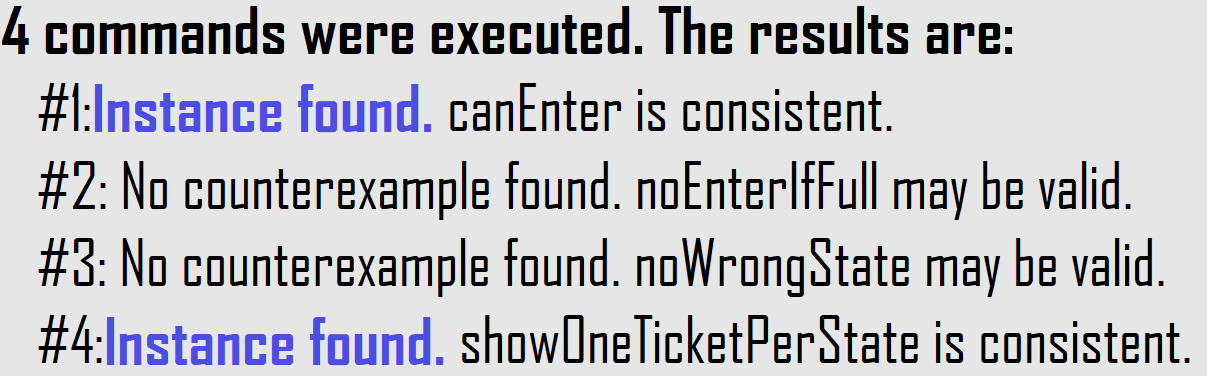
\includegraphics[width=0.6\textwidth] {alloy/alloyrun}
	\caption{Alloy analysis results}
	\label{run} 
\end{figure}

The generated world can be seen in Figure \ref{metamodel}, while Figure \ref{oneforstate} offers an example where exists a ticket for each consistent state (Non-relevant signatures are hidden in Figure \ref{oneforstate_compl}).

\begin{landscape}
	\begin{figure}[p]	
		\centering
		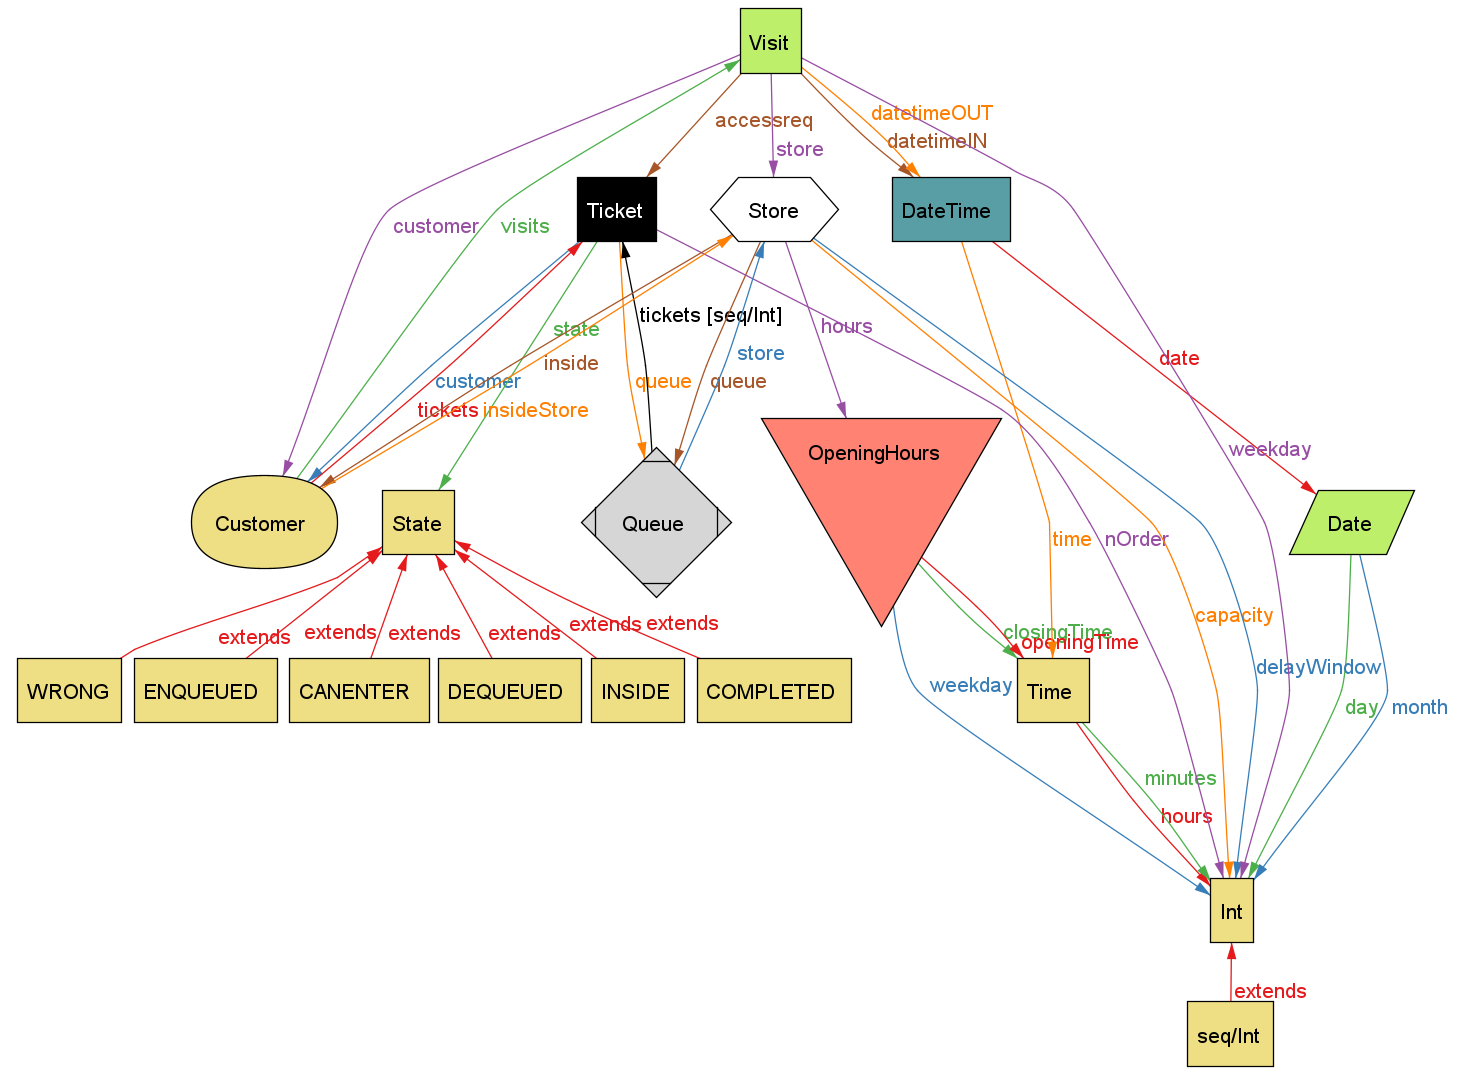
\includegraphics[height=\textheight] {alloy/metamodel}
		\caption{Alloy metamodel}
		\label{metamodel} 
	\end{figure}
	
	\begin{figure}[p]
		\centering	
		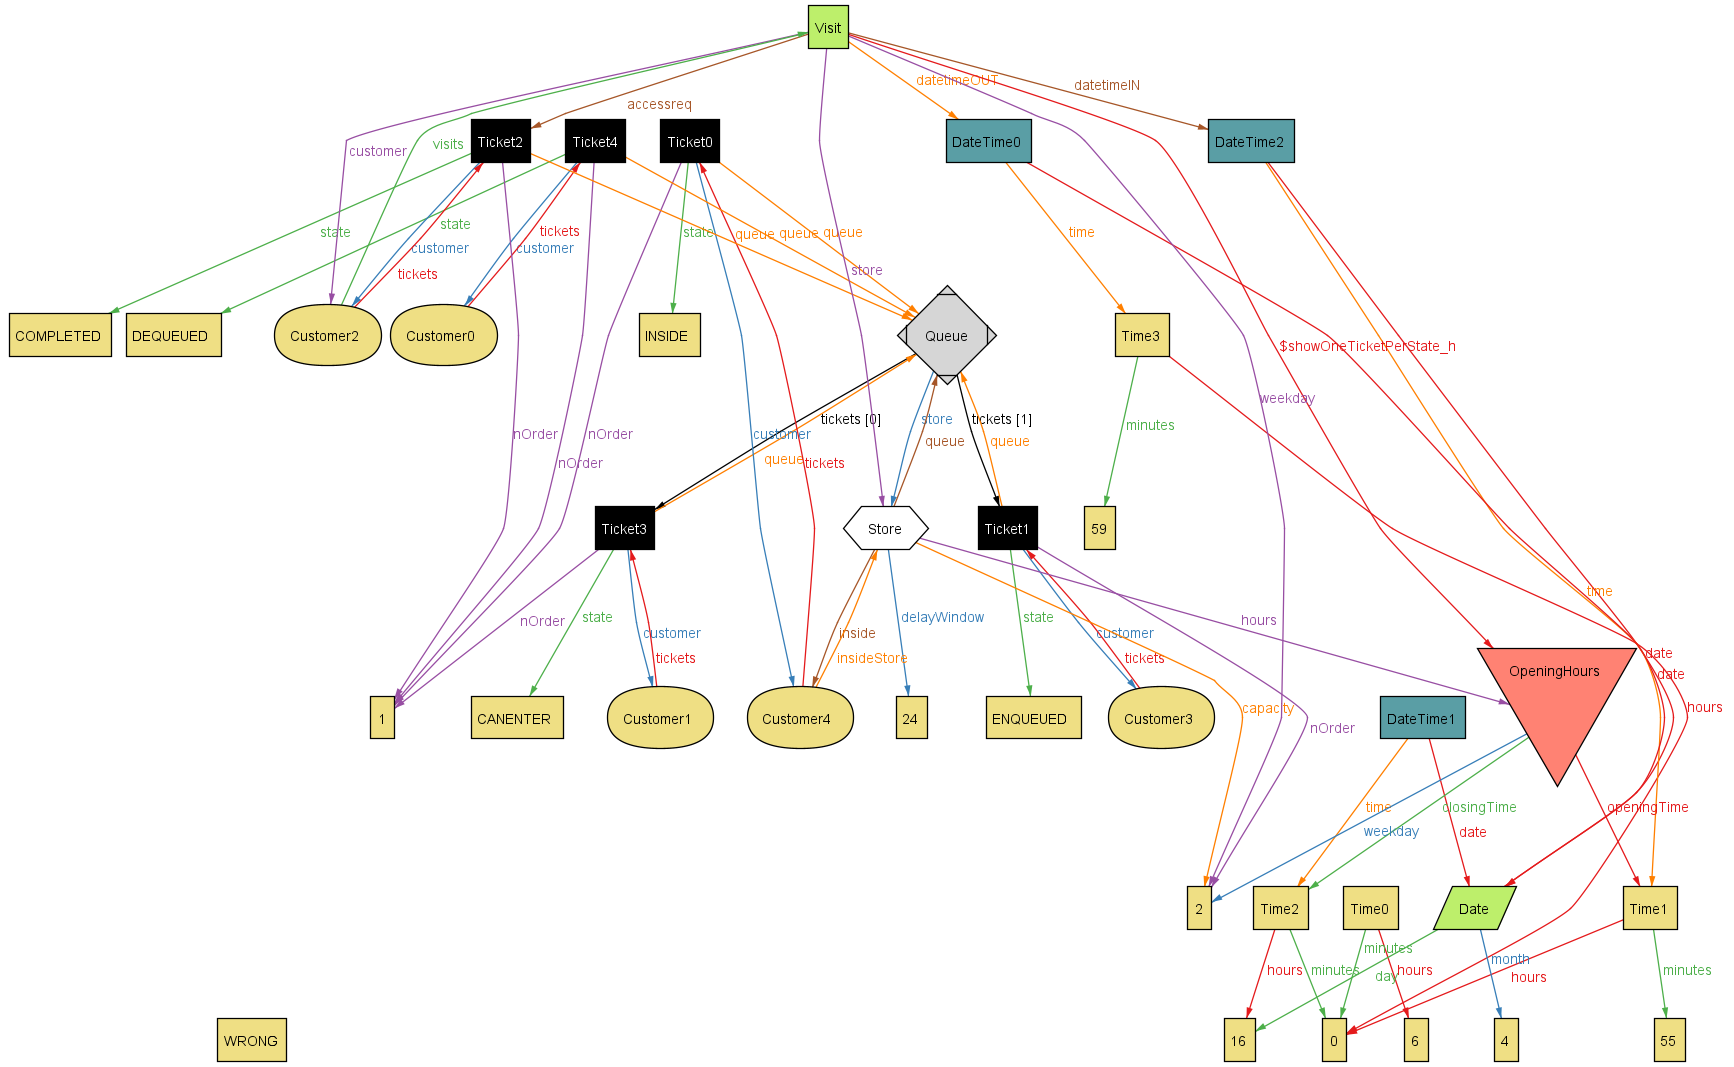
\includegraphics[width=\linewidth] {alloy/1perstate_complete}
		\caption{Result of running \texttt{showOneTicketPerState}}
		\label{oneforstate} 
	\end{figure}
	
	\begin{figure}[p]	
		\centering
		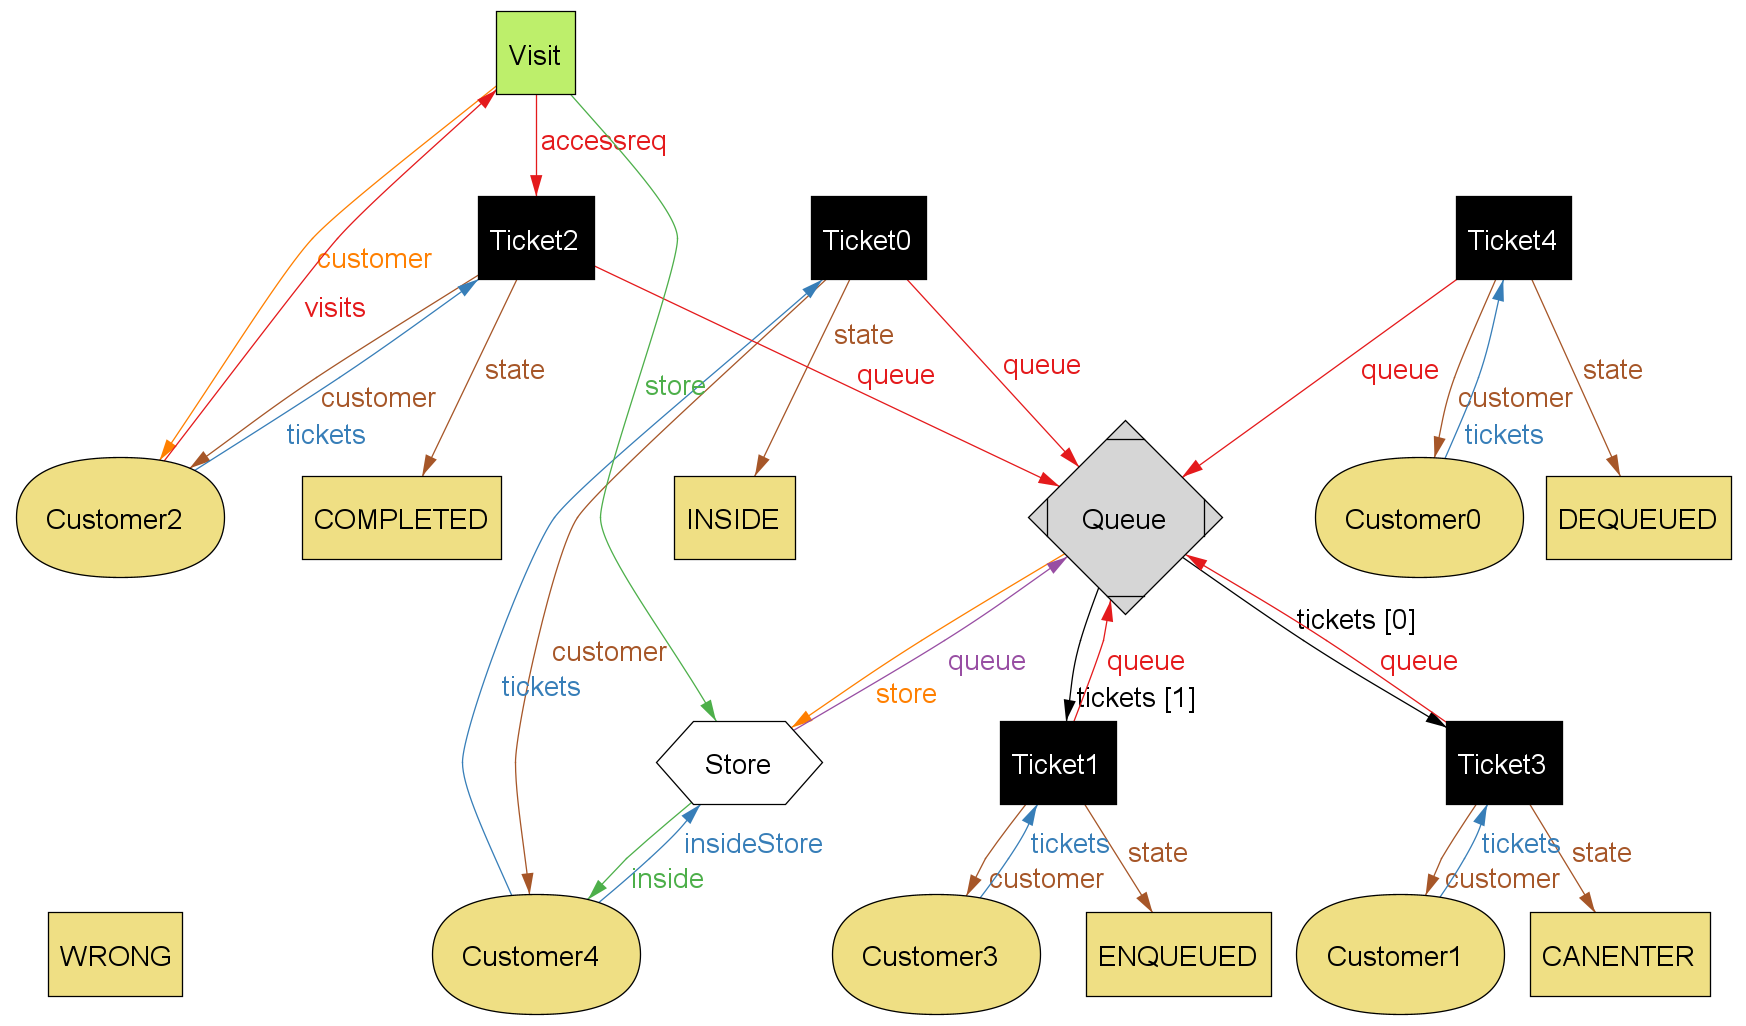
\includegraphics[width=0.8\linewidth] {alloy/1perstate}
		\caption{Result of running \texttt{showOneTicketPerState} (Only relevant signatures)}
		\label{oneforstate_compl} 
	\end{figure}
\end{landscape}
